

\StartOf{Lecture 4}

\Today{(1) Fourier Transform and Bandwidth, (2) Sampling Intro}

\announcements{
\begin{itemize}
\item Guest lecture today: Dr. Alemayehu Solomon Abrar
\item Homework 1 due Wed Jan 29 at 11:59pm.  Accepted 24 hours late with 10\% penalty.  Solutions will be posted Thu night just after midnight.
\item Homework 2 posted today, due Wed Feb 5 at 11:59pm.
\item Reading: Today -- Rice 2.4-2.7 and 6.2.1; Next -- Appendix A.2
\end{itemize}
}

So far we've been talking about continuous-time waveforms.  We just had a lecture on signal space representations, which is a discrete representation of a continuous-time signal.  But we have not talked specifically about discrete-time signals, nor have we talked about the bandwidth of the waveforms we are using.

Today's objectives are to provide the tools needed to study:
\begin{enumerate}
 \item The frequency content of waveforms that we will use for digital communications systems,
 \item Sampling of continuous-time signals, and the frequency content of discrete-time signals, and
 \item Operations we will do on discrete-time signals, for example, frequency translation and filtering.
\end{enumerate}

\section{Fourier Transform}

The Fourier transform (FT) is a transform used to show the frequency content of continuous-time, aperiodic signals.

\begin{table}
 \begin{tabular}{|l|cc|}
  \hline
  & \multicolumn{2}{c|}{\bf Periodicity:} \\
  \bf Time:                         & \textit{Periodic} & \textit{Aperiodic} \\
\hline
\textit{Continuous-Time} &                             & \underline{Laplace Transform} \\
                         &                             & $x(t) \leftrightarrow X(s)$ \\
                         & \underline{Fourier Series}  & \underline{Fourier Transform} \\
                         & $x(t) \leftrightarrow a_k$  & $x(t) \leftrightarrow X(j\omega)$ \\
                         &                             & $X(j\omega) = \int_{t=-\infty}^\infty x(t) e^{-j\omega t} dt$ \\
                         &                             & $x(t) = \frac{1}{2\pi} \int_{\omega=-\infty}^\infty X(j\omega) e^{j\omega t} d\omega$ \\
\hline
\textit{Discrete-Time}   &                                  & \underline{z-Transform}  \\
                         &                                  & $x(n) \leftrightarrow X(z)$ \\
                         & \underline{Discrete Fourier Transform (DFT)} & \underline{Discrete Time Fourier Transform (DTFT)} \\
                         & $x(n) \leftrightarrow X[k]$      & $x(n) \leftrightarrow X(e^{j\Omega})$ \\
                         & $X[k] = \sum_{n=0}^{N-1} x(n) e^{-j\frac{2\pi}{N} kn}$
                                                            & $X(e^{j\Omega}) = \sum_{n=-\infty}^\infty x(n) e^{-j\Omega n}$ \\
                         & $x(n) = \frac{1}{N} \sum_{k=0}^{N-1} X[k] e^{j\frac{2\pi}{N} nk}$
                                                            & $x(n) = \frac{1}{2\pi} \int_{n=-\pi}^\pi X(e^{j\Omega}) d\Omega$ \\
\hline
 \end{tabular} 
\caption{Frequency Transforms}
\end{table} 


Notes about continuous-time frequency transforms:
\begin{enumerate}
 \item You might be most familiar with the Laplace Transform.  To convert it to the Fourier transform, we replace $s$ with $j \omega$, where   $\omega$ is the radial frequency, with units radians per second (rad/s).
 \item You may prefer the radial frequency representation, but also feel free to use the rotational frequency $f$ (which has units of cycles per sec, or Hz.  Frequency in Hz is more standard for communications; you should use it for intuition.  In this case, just substitute $\omega = 2\pi f$.  You could write $X(j2\pi f)$ as the notation for this, but typically you'll see it written as $X(f)$.  Note that the definition of the Fourier transform in the $f$ domain removes the $\frac{1}{2\pi}$ in the inverse Fourier transform definition.
   \begin{eqnarray}
     X(j2\pi f) &=& \int_{t=-\infty}^\infty x(t) e^{-j 2\pi f t} dt \nonumber \\
     x(t) &=&  \int_{f=-\infty}^\infty X(j2\pi f) e^{j2\pi f t} df \nonumber 
   \end{eqnarray}
 \item The Fourier series is limited to purely periodic signals.  Both Laplace and Fourier transforms are \textit{not} limited to periodic signals.
 \item Note that $e^{j\alpha} = \cos(\alpha) + j \sin(\alpha)$.
\end{enumerate}

See Table 2.4.4 in the Rice book.

\Example{Square Wave}{ Given a rectangular pulse $x(t) =
\rect(t/T_s)$,
\[
x(t) = \pdfarray{1}{-T_s/2 < t \le T_s/2}
\]
What is the Fourier transform $X(f)$?  Calculate both from the
definition and from a table.

\Solution{ Method 1:  From the definition:
\begin{eqnarray}
  X(j\omega) &=& \int_{t=-T_s/2}^{T_s/2} e^{-j\omega t} dt \nonumber \\
       &=& \left. \frac{1}{-j\omega} e^{-j\omega t}
           \right|_{t=-T_s/2}^{T_s/2} \nonumber \\
       &=& \frac{1}{-j\omega} \left(e^{-j\omega T_s/2} - e^{j\omega T_s/2} \right)
           \nonumber 
\end{eqnarray}
Using the fact that $\frac{1}{-2j}\left(e^{-j\alpha} -
e^{j\alpha} \right) = \sin (\alpha)$, we have:
\[
  X(j\omega)= 2 \frac{\sin(\omega T_s/2) }{\omega}  = T_s \frac{\sin(\omega T_s/2) }{\omega T_s/2}. \nonumber
\]
While it is sometimes convenient to replace $\frac{\sin (\pi x)}{\pi x}$ with $\sinc (x)$, it is confusing because $\sinc (x)$ is sometimes defined as $\frac{\sin(\pi x)}{\pi x}$ and sometimes defined as $\frac{\sin x}{x}$.  No standard definition for `sinc' exists!  Rather than make a mistake because of this, the Rice book always writes out the expression fully.  I will try to follow suit. \\

Method 2: From the tables and properties.  Let $T=T_s/2$.  Then
\begin{equation}
 x(t) = \pdfarray{1}{|t|<T},
\end{equation}
which is in Table 2.4.4.  From the table, 
\[
X(j\omega) = 2T \frac{\sin (\omega T)}{\omega T} =  T_s \frac{\sin (\omega T_s/2)}{\omega T_s/2}.
\]
}

See Figure \ref{F:plotSinc}(a).
\begin{figure}[htbp]
(a)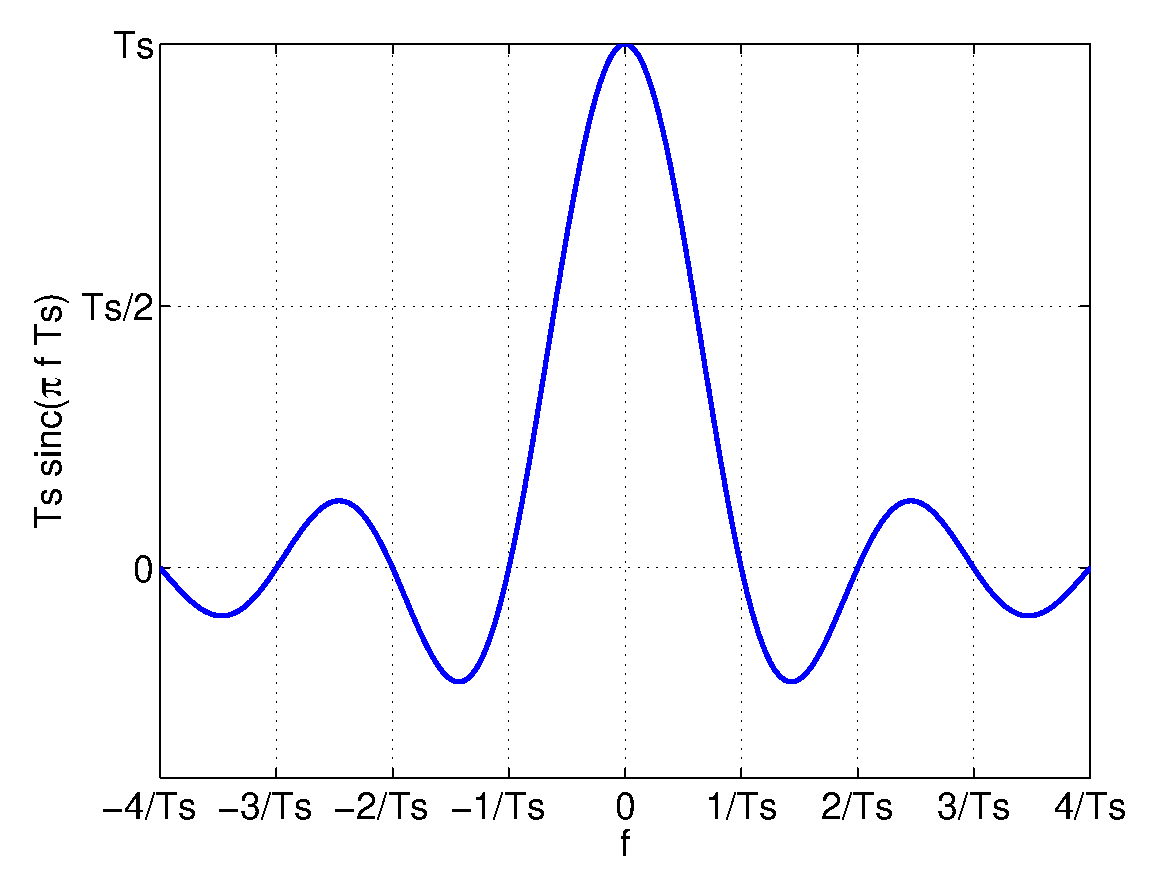
\includegraphics[width=0.45\textwidth]{../images/plotSinc.eps}(b)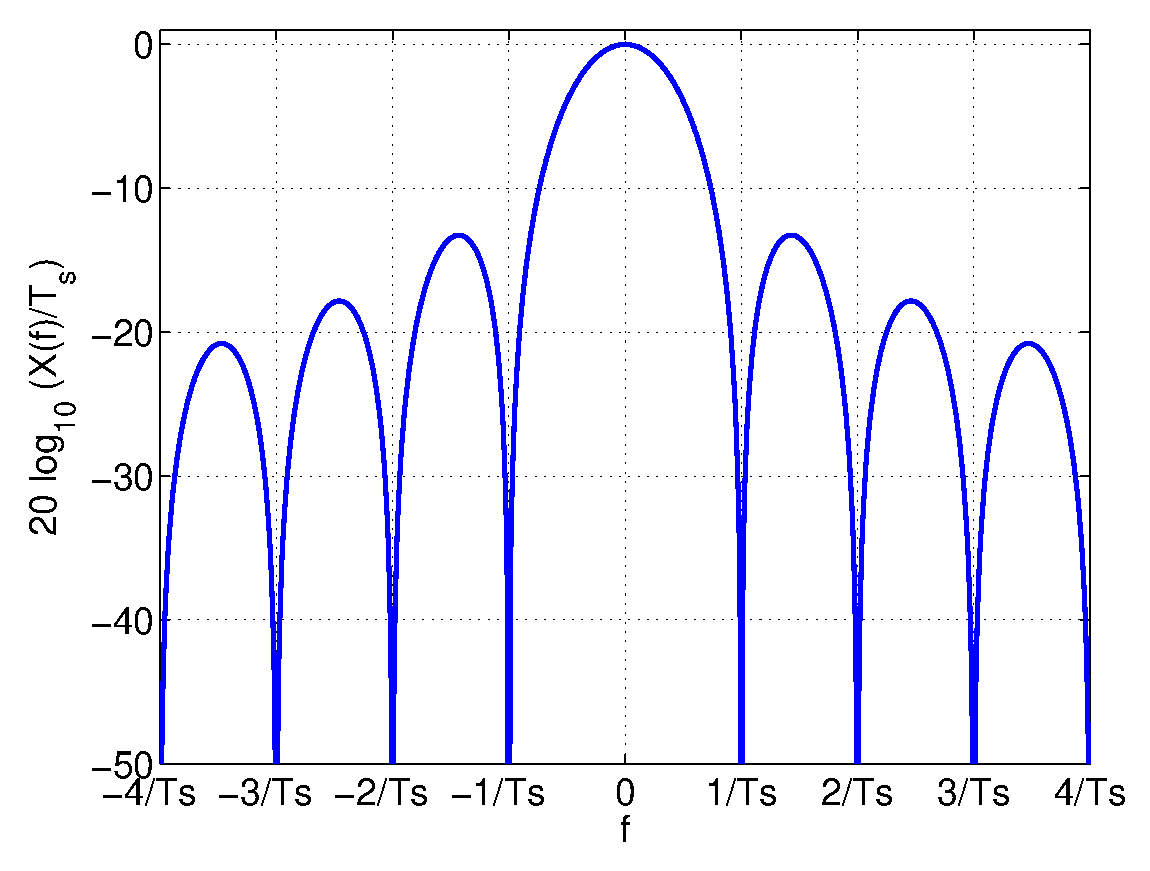
\includegraphics[width=0.45\textwidth]{../images/plotSincPowerdB.eps}
  \caption{(a) Fourier transform $X(j2\pi f)$ of rect pulse with period $T_s$, and (b) Power vs.\ frequency $20\log_{10}(X(j2\pi f)/T_s)$.}
  \label{F:plotSinc}
\end{figure}


\Question  What if $Y(j\omega)$ was a rect function?  What would the
inverse Fourier transform $y(t)$ be?

One can see a problem of using waveforms that are rectangular-shaped in \emph{either} the time or frequency domains.  If 100\% limited in the time domain, then the signal spreads infinitely in frequency; if 100\% limited in the frequency domain, then the signal spreads out infinitely in time.

\subsection{Fourier Transform Properties}

See Table 2.4.3 in the Rice book.

Assume that $\Fourier{x(t)} = X(j\omega)$.  Important properties of the
Fourier transform:
\begin{enumerate}
  \item Time shift property:
     \[
       \Fourier{x(t-t_0)} = e^{-j\omega t_0} X(j\omega)
     \]
  \item Scaling property: for any real $a\neq 0$,
     \[
       \Fourier{x(at)} = \frac{1}{|a|} X \left( j\frac{\omega}{a}\right)
     \]
  \item Convolution property: if, additionally $y(t)$ has Fourier
  transform $X(j\omega)$,
     \[
       \Fourier{x(t) \star y(t)} = X(j\omega) \cdot Y(j\omega)
     \]
  \item Modulation property:
     \[
       \Fourier{x(t) cos(\omega_0 t)} = \frac{1}{2}X(\omega-\omega_0)+ \frac{1}{2}X(\omega + \omega_0)
     \]
  \item Duality property:
     \begin{eqnarray}
       x(j\omega) &=& \Fourier{X(-t)} \nonumber \\
       x(-j\omega) &=& \Fourier{X(t)} \nonumber
     \end{eqnarray}
     This says is that you can go backwards in a Fourier transform table -- Replace the $\omega$ with $t$ in the frequency column, and replace $t$ with $-\omega$ in the time-domain column.
  \item Parceval's theorem:  The energy calculated in the frequency
  domain is equal to the energy calculated in the time domain.
     \[
       \int_{t=-\infty}^\infty |x(t)|^2 dt = \int_{f=-\infty}^\infty |X(f)|^2  df = \frac{1}{2\pi}\int_{\omega=-\infty}^\infty |X(j\omega)|^2 d\omega
     \]
     So do whichever one is easiest!  Or, check your answer by doing
     both.
\end{enumerate}

\Example{Applying FT Properties} If $w(t)$ has the Fourier transform $W(j \omega)$, find $X(j \omega)$ for the following:  $x(t) = w(2t + 2)$.

\Solution{
Let $x(t) = z(2t)$ where $z(t) = w(t+2)$.  Then $Z(j \omega) = e^{j2\omega} W(j \omega)$.  Then $X(j \omega) = \frac{1}{2}Z\left( \frac{j \omega}{2} \right)$.  So plugging in the first result,
  \[
   X(j \omega) = \frac{1}{2} e^{j\omega} W\left( \frac{j \omega}{2} \right).
  \]
  Alternatively, let $x(t) = y(t+1)$ where $y(t) = w(2t)$.  Then $X(j \omega) = e^{j\omega} Y(j \omega)$.  Then $Y(j \omega) = \frac{1}{2}W\left( \frac{j \omega}{2} \right)$.  Plugging in,
  \[
   X(j \omega) = e^{j\omega} \frac{1}{2}W \left( \frac{j \omega}{2} \right).
  \]
  The two approaches come up with the same answer, as they should.
}



\subsection{Bandwidth}

Bandwidth is a critical resource for a digital communications system; we have various definitions to quantify it.  In short, it isn't easy to describe a signal in the frequency domain with a single number.  And, in the end, a system will be designed to meet a spectral mask required by the FCC or system standard.

Intuitively, bandwidth is the maximum extent of our signal's frequency domain characterization $X(f)$.  A baseband signal absolute bandwidth is often defined as the $W$ such that $X(f)=0$ for all $f$ except for the range $-W \le f \le W$.  Other definitions for bandwidth are 
\begin{itemize}
 \item 3-dB bandwidth: $B_{3dB}$ is the value of $f$ such that $|X(f)|^2 = |X(0)|^2/2$.
 \item 90\% bandwidth: $B_{90\%}$ is the narrowest range which captures 90\% of the energy in the signal:
\[
  \int_{-B_{90\%}}^{B_{90\%}} |X(f)|^2 df = 0.90 \intinfty{f}{|X(f)|^2}
\]
\end{itemize}

As a motivating example, I mention the square-root raised cosine (SRRC) pulse, which has the following desirable Fourier transform:
\begin{equation} \label{E:RRC}
H_{RRC}(f) = \pdfarrays{\sqrt{T_{s}}}{0 \le |f| \le
\frac{1-\alpha}{2T_{s}}}
                      {\sqrt{\frac{T_{s}}{2}\left\{ 1 + \cos \left[
                      \frac{\pi T_{s}}{\alpha} \left( |f| - \frac{1-\alpha}{2T_{s}}
                       \right)\right]\right\}}}{ \frac{1-\alpha}{2T_{s}} \le |f| \le
                       \frac{1+\alpha}{2T_{s}}}
\end{equation}
where $\alpha$ is a parameter called the ``rolloff factor''.  We can actually analyze this using the properties of the Fourier transform and many of the standard transforms you'll find in a Fourier transform table.

The SRRC and other pulse shapes are discussed in Appendix A, and we will go into more detail later on.  The purpose so far is to motivate practicing up on frequency transforms. 

\Example{Butterworth Filter} 
A Butterworth low-pass filter has a frequency response with magnitude,
\[
|H(f)| = \frac{1}{\sqrt{1 + (f/f_0)^{2n}}}
\]
where $n$ is the number of reactive components (\ie, inductors or
capacitors).
  \begin{enumerate}
    \item What is the 3dB bandwidth of this filter?
    \item Find the lowest $n$ so that $|H(f)|^2$ is constant to within 1
    dB over the frequency range $-0.8 f_0 < f < 0.8 f_0$.  Hint:
    $|H(f)|^2$ is strictly decreasing as $|f|$ increases.  So the requirement
    is that $|H(0)|^2$ is no more than 1.26 times $|H(0.8 f_0)|^2$.
  \end{enumerate}

\Solution{  
\begin{enumerate}
    \item The squared magnitude, $|H(f)|^2$ is equal to 1/2 when $f=f_0$, regardless of $n$.  Thus the 3dB bandwidth is always $f_0$.
    \item  $|H(f)|$ is strictly decreasing from $f=0$.  We need to find the
      $n$ such that $|H(\pm 0.8 f_0)|^2$ is more than 1 dB down from
      the filter's maximum value (at $f=0$).  Note that
      \[
        10 \log_{10} |H(f)|^2 = -10 \log_{10} \left( 1 + (f/f_0)^{2n}\right)
      \]
      which makes $10 \log_{10} |H(0)|^2 = 0$ and thus we are looking for the $n$ that
      has:
      \begin{eqnarray}
        -1 &=& 10 \log_{10} |H(0.8 f_0)|^2 = - 10 \log_{10}(1+0.8^{2n})
          \nonumber \\
       0.1 &=& \log_{10} (1+0.8^{2n})
          \nonumber \\
       10^{0.1} - 1 &=& 0.8^{2n}
          \nonumber \\
       n &=& \frac{ \log(10^{0.1} - 1)}{2 \log(0.8)} \approx 3.03
          \nonumber
      \end{eqnarray}
      While $n=3$ is a good engineering answer, $n=4$ is a good math answer, since $n=3$, technically, would lead to $> 1$ dB variation.
  \end{enumerate}
}


\subsection{Linear Time Invariant (LTI) Filters}

If a (deterministic) signal $x(t)$ is input to a LTI filter with
impulse response $h(t)$, the output signal is
\[
  y(t) = h(t) \star x(t)
\]
Using the above convolution property,
\[
  Y(j \omega) = X(j \omega)  H(j \omega)
\]

\section{Sampling}

A common statement of the Nyquist sampling theorem is that a signal
can be sampled at twice its bandwidth.  But the theorem really has
to do with signal reconstruction from a sampled signal.

\Theorem{(Nyquist Sampling Theorem.) Let $x_c(t)$ be a baseband,
continuous signal with bandwidth $B$ (in Hz), \ie, $X_c(j\omega) = 0$ for
all $|\omega| \ge 2\pi B$. Let $x_c(t)$ be sampled at multiples of
$T$, where $\frac{1}{T} \ge 2B$ to yield the sequence
$\{x_c(nT) \}_{n=-\infty}^\infty $. Then
\begin{equation} \label{E:NyquistSamplingTheorem}
  x_c(t) = 2BT \sum_{n=-\infty}^\infty x_c(nT)
  \frac{\sin (2\pi B(t-nT))}{2\pi B(t-nT)}.
\end{equation}}
{Not covered.}

Notes:
\begin{itemize}
\item This is an interpolation procedure.
\item This is a synthesis equation with $\frac{\sin (2\pi B(t-nT))}{2\pi B(t-nT)}$ waveforms as the orthogonal basis functions.
\item This is only precise when $X(j\omega) = 0$ for all $|\omega| \ge 2\pi B$.
\end{itemize}

\subsection{Aliasing Due To Sampling}

Essentially, sampling is the multiplication of a impulse train (at
period $T$ with the desired signal $x(t)$:
\begin{eqnarray} \label{E:SampledViaImpulseTrain}
  x_{sa}(t) &=&  x(t) \sum_{n=-\infty}^\infty \delta(t-nT) \nnn
  x_{sa}(t) &=&  \sum_{n=-\infty}^\infty x(nT)  \delta(t-nT) \nn
\end{eqnarray}

What is the Fourier transform of $x_{sa}(t)$?  In the frequency domain, this is a convolution:
\begin{eqnarray} \label{E:FT_of_Sampled_Signal_1}
  X_{sa}(j\omega) &=& X(j\omega) \star \frac{2\pi}{T} \sum_{n=-\infty}^\infty \delta\left(\omega- \frac{2\pi n}{T} \right)
    \nonumber \\
  &=& \frac{1}{T}  \sum_{n=-\infty}^\infty X\left(j \left( \omega- \frac{2\pi n}{T}
  \right) \right) \quad \mbox{for all } \omega
    \\
  &=& \frac{1}{T}  X(j\omega) \quad \mbox{for } |\omega| < 2\pi B \mbox{ if } X(j\omega) \mbox{is bandlimited.}
    \nonumber
\end{eqnarray}}

This is shown graphically in the Rice book in Section 2.6.1 ``The Sampling Theorem'', Figure 2.12.

The Fourier transform of the sampled signal is many copies of $X(j\omega)$
strung at integer multiples of $2\pi /T$, as shown in
Fig.~\ref{F:Sampling-FreqDomain}.

\begin{figure}[htbp]
  \centerline{ 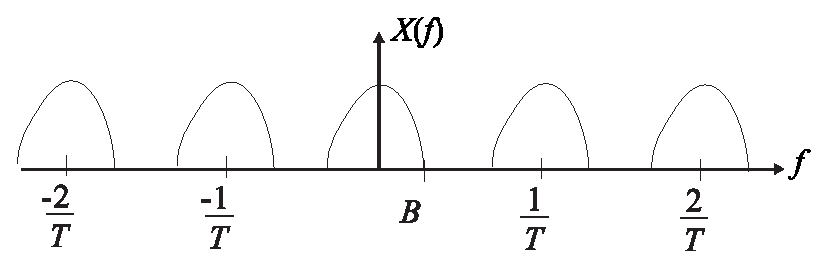
\includegraphics[width=0.65\textwidth]{../images/Sampling-FreqDomain_bandwidthB_f.eps}}
  \caption{The effect of sampling on the frequency spectrum in terms of frequency $f$ in Hz.}
  \label{F:Sampling-FreqDomain}
\end{figure}

\Example{Sinusoid sampled above and below Nyquist rate} Consider two
sinusoidal signals sampled at $1/T = 25$ Hz:
\begin{eqnarray}
  x_1(nT) &=& \sin(2 \pi 5 n T) \nnn
  x_2(nT) &=& \sin(2 \pi 20 n T) \nn
\end{eqnarray}
What are the two frequencies of the sinusoids, and what is the
Nyquist rate?  Which of them does the Nyquist theorem apply to? Draw
the spectrums of the continuous signals $x_1(t)$ and $x_2(t)$, and
indicate what the spectrum is of the sampled signals.

Figure \ref{F:NyquistInterpolations_SinusoidalSignals} shows what
happens when the Nyquist theorem is applied to the each signal
(whether or not it is valid).  What observations would you make
about Figure \ref{F:NyquistInterpolations_SinusoidalSignals}(b),
compared to Figure
\ref{F:NyquistInterpolations_SinusoidalSignals}(a)?

\begin{figure}[htbp]
  (a)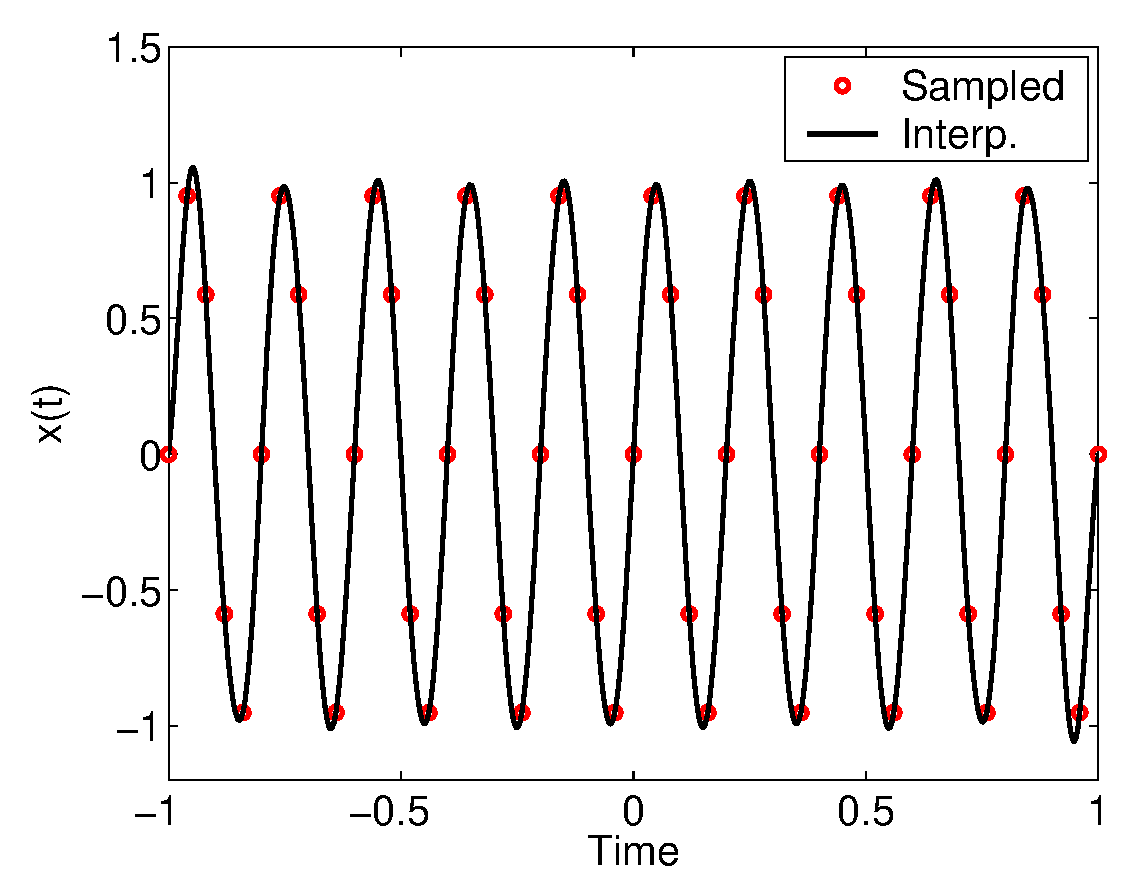
\includegraphics[width=0.45\textwidth]{../images/plotInterpolatedSin_f5.eps}(b)\includegraphics[width=0.45\textwidth]{../images/plotInterpolatedSin_f20.eps}
  \caption{Sampled (a) $x_1(nT)$ and (b) $x_2(nT)$ are interpolated (---) using the Nyquist interpolation formula.}
  \label{F:NyquistInterpolations_SinusoidalSignals}
\end{figure}


\Example{Square vs.\ round pulse shape} Consider the square pulse
considered before, $x_1(t) = \rect(t/T_s)$.  Also consider a
parabola pulse (this doesn't really exist in the wild -- I'm making it up for an example.)
\[
  x_2(t) = \pdfarray{1- \left(\frac{2t}{T_s}\right)^2}
                    {-\frac{1}{2T_s} \le t \le \frac{1}{2T_s}}
\]
What happens to $x_1(t)$ and $x_2(t)$ when they are sampled at rate
$T$?

\begin{figure}[htbp]
  (a)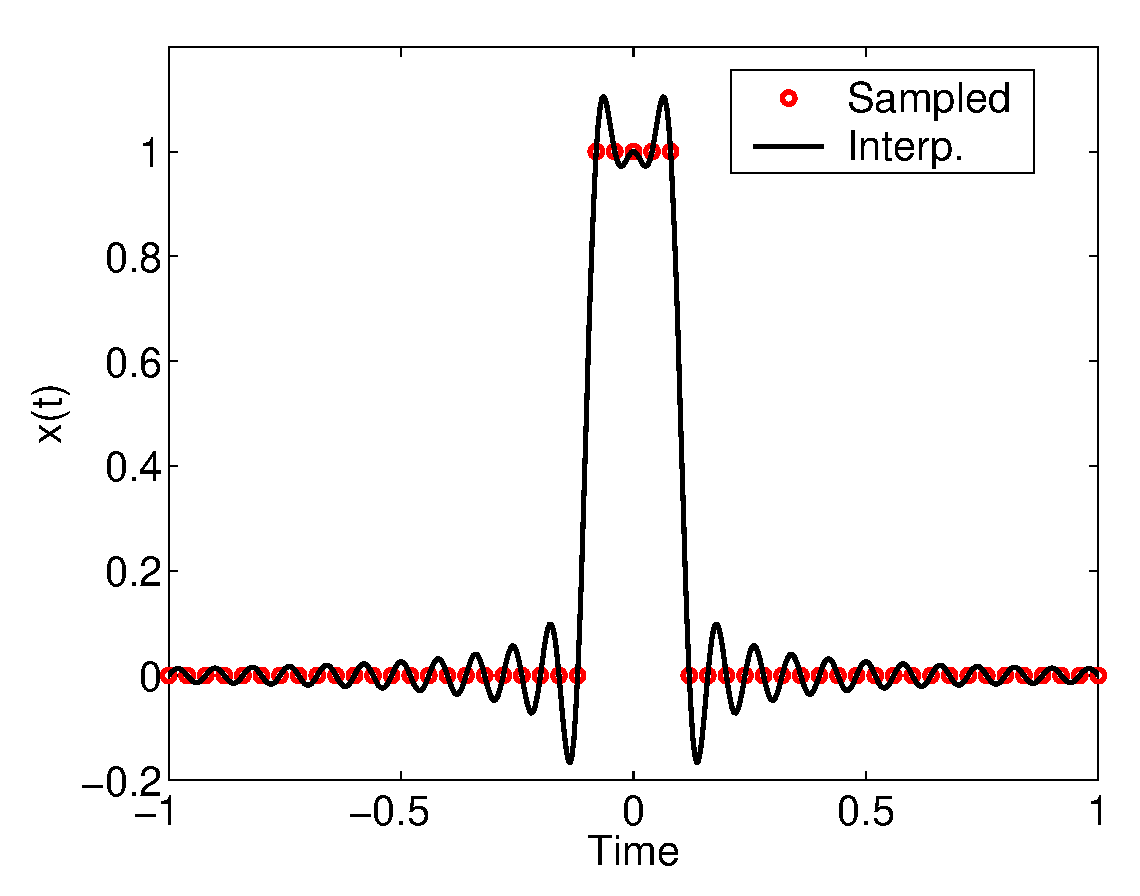
\includegraphics[width=0.45\textwidth]{../images/plotEgNyquistInterpolation_SquarePulse.eps}(b)\includegraphics[width=0.5\textwidth]{../images/plotEgNyquistInterpolation_ParabolaPulse.eps}
  \caption{Sampled (a) $x_1(nT)$ and (b) $x_2(nT)$ are interpolated (---) using the Nyquist interpolation formula.}
  \label{F:NyquistInterpolations}
\end{figure}

In the Matlab code \texttt{EgNyquistInterpolation.m}  we set
$T_s=1/5$ and $T=1/25$.  Then, the sampled pulses are
interpolated using (\ref{E:NyquistSamplingTheorem}). Even though
we've sampled at a pretty high rate, the reconstructed signals will
not be perfect representations of the original, in particular for
$x_1(t)$.  See Figure \ref{F:NyquistInterpolations}.


% \subsection{Connection to DTFT}
% 
% Recall (\ref{E:SampledViaImpulseTrain}).  We calculated the Fourier
% transform of the product by doing the convolution in the frequency
% domain.  Instead, we can calculate it directly from the formula.
% 
% \begin{eqnarray} \label{E:FT_of_sampledSignal}
%   X_{sa}(j \omega) &=&  \int_{t=-\infty}^\infty \sum_{n=-\infty}^\infty x(nT)  \delta(t-nT) e^{-j\omega t}
%   \nnn
%     &=&  \sum_{n=-\infty}^\infty x(nT)  \int_{t=-\infty}^\infty  \delta(t-nT) e^{-j\omega t}
%   \\
%     &=&  \sum_{n=-\infty}^\infty x(nT)  e^{-j\omega n T}
%   \nn
% \end{eqnarray}
% 
% The discrete-time Fourier transform of $x_{sa}(t)$, I denote
% $\DTFT{x_{sa}(t)}$, and it is:
% \[
%  \DTFT{x_{sa}(t)} =  X_{d}(e^{j\Omega}) = \sum_{n=-\infty}^\infty x(nT)  e^{-j\Omega n}
% \]
% Essentially, the difference between the DTFT and the Fourier
% transform \emph{of the sampled signal} is the relationship
% \[
%  \Omega =  \omega T = 2\pi f T
% \]
% 
% But this defines the relationship only between the Fourier transform
% of the sampled signal.  How can we relate this to the FT of the
% continuous-time signal?  A: Using (\ref{E:FT_of_Sampled_Signal_1}). We
% have that $X_{d}(e^{j\omega}) = X_{sa}\left( \frac{\Omega}{T}\right)$.  Then plugging into (\ref{E:FT_of_Sampled_Signal_1}),
% \begin{eqnarray}
%   X_{d}(e^{j\Omega}) &=& X_{sa}\left( j \frac{\Omega}{T}\right)
%   \nnn
%    &=&  \frac{1}{T}  \sum_{n=-\infty}^\infty X\left(j \left( \frac{\Omega}{T} - \frac{2\pi n}{T}
%   \right) \right) \nnn
%    &=&  \frac{1}{T}  \sum_{n=-\infty}^\infty X\left(j \left( \frac{\Omega - 2\pi n}{T}
%   \right) \right) \nnn
% \end{eqnarray}
% 
% 
%  If $x(t)$ is sufficiently bandlimited, $X_{d}(e^{j\Omega}) \propto X(j\Omega/T)$
% in the interval $-\pi < \Omega < \pi$. This relationship holds for the Fourier transform of the original,
% \emph{continuous-time signal} between $-\pi < \Omega < \pi$
% \textbf{if and only if} the original signal $x(t)$ is sufficiently
% \textbf{bandlimited} so that the Nyquist sampling theorem applies.
% 
% 
% Notes:
% \begin{itemize}
%   \item Most things in the DTFT table in Table 2.4.8 are analogous to continuous functions which are not bandlimited.  So - don't expect the last form to apply to any continuous function.
%   \item The DTFT is periodic in $\Omega$ with period $2\pi$.
%   \item Don't be confused:  The DTFT is a continuous function of  $\Omega$.
% \end{itemize}
% 
% 
% 
% 
